\documentclass[12pt]{article} % use larger type; default would be 10pt
\usepackage[czech]{babel}
\usepackage[utf8]{inputenc} % set input encoding (not needed with XeLaTeX)

%%% PAGE DIMENSIONS
\usepackage{geometry} % to change the page dimensions
% \usepackage[left=2cm,right=2cm,top=2cm,bottom=2cm]{geometry}
\geometry{a4paper}
% \geometry{margin=2in} % for example, change the margins to 2 inches all round
% \geometry{landscape} % set up the page for landscape

\usepackage{graphicx} % support the \includegraphics command and options
\usepackage{wrapfig} % support the wrapfigure section

\usepackage{tikz} % graphs
\usepackage{pgfplots}

\usepackage{hyperref} % links in \tableofcontents
\hypersetup{
	colorlinks,
	citecolor=black,
	filecolor=black,
	linkcolor=black,
	urlcolor=black
}

% \usepackage[parfill]{parskip} % Activate to begin paragraphs with an empty line rather than an indent

%%% PACKAGES
\usepackage{booktabs} % for much better looking tables
\usepackage{array} % for better arrays (eg matrices) in maths
% \usepackage{paralist} % very flexible & customisable lists (eg. enumerate/itemize, etc.)
\usepackage{verbatim} % adds environment for commenting out blocks of text & for better verbatim
\usepackage{subfig} % make it possible to include more than one captioned figure/table in a single float
% These packages are all incorporated in the memoir class to one degree or another...
\usepackage{float}

%%% HEADERS & FOOTERS
\usepackage{fancyhdr} % This should be set AFTER setting up the page geometry
\pagestyle{fancy} % options: empty , plain , fancy
\renewcommand{\headrulewidth}{0pt} % customise the layout...
\lhead{}\chead{}\rhead{}
\lfoot{}\cfoot{\thepage}\rfoot{}

%%% SECTION TITLE APPEARANCE
\usepackage{sectsty}
\allsectionsfont{\sffamily\mdseries\upshape} % (See the fntguide.pdf for font help)
% (This matches ConTeXt defaults)

%%% ToC (table of contents) APPEARANCE
\usepackage[nottoc,notlof,notlot]{tocbibind} % Put the bibliography in the ToC
\usepackage[titles,subfigure]{tocloft} % Alter the style of the Table of Contents
\renewcommand{\cftsecfont}{\rmfamily\mdseries\upshape}
\renewcommand{\cftsecpagefont}{\rmfamily\mdseries\upshape} % No bold!
\newcommand{\bigsize}{\fontsize{35pt}{20pt}\selectfont}

%%% END Article customizations

\begin{document}
\begin{titlepage}
	
\includegraphics[scale=0.7]{logo.jpg}
	\vspace*{\fill}
	\begin{center}
		\textsc{\LARGE \bigsize Parametry zdroje napětí}\\[1cm]
		Martin Zlámal \\[1cm]
		{\small\em \copyright \ Datum poslední revize \today } \\
		\LaTeX
	\end{center}
	\vspace*{\fill}
\end{titlepage}
\tableofcontents
\listoffigures
\listoftables
\newpage

\section{Zadání}
\begin{enumerate}
\item Změřte zatěžovací charakteristiku $U=f(I)$ baterie.
\item Grafickou extrapolací změřených hodnot určete napětí naprázdno ($U_0$) a proud nakrátko ($I_k$).
\item Určete vnitřní odpor baterie ($R_i$).
\item Dopočítejte výkonovou charakteristiku $P=f(R_z/R_i)$.
\item Stanovte při kterém odporu zátěže dává baterie maximální výkon.
\end{enumerate}

\section{Teoretický úvod}
Následuje vysvětlení několika základních pojmů.
\begin{description}
\item[Ideální zdroj napětí] \hfill \\ Ideální napěťový zdroj udržuje na svých svorkách dané napětí, nezávisle na odebíraném proudu. Vnitřní odpor ideálního zdroje napětí $R_i=0\Omega$.
\item[Reálný zdroj napětí] \hfill \\ Reálný zdroj napětí má určitý vnitřní odpor, na kterém vzniká úbytek napětí a výstupní napětí klesá.
\item[Ideální zdroj proudu] \hfill \\ Ideální proudový zdroj dodává do obvodu konstantní proud nezávisle na napětí, které je třeba vyvinout. Vnitřní odpor ideálního zdroje proudu je $R_i=\infty\Omega$.
\item[Reálný zdroj proudu] \hfill \\ Reálný zdroj proudu nedosahuje nekonečné hodnoty vnitřního odporu, takže na tomto vnitřím odporu vznikají ztráty.
\item[Zatěžovací charakteristika zdroje] \hfill \\ Zatěžovací charakteristika zdroje je grafická závislost napětí na svorkách zdroje vzhledem k odebíranému proudu z tohoto zdroje.
\item[Napětí naprázdno, proud nakrátko] \hfill \\ Jedná se o speciální případy zapojení zapojení obvodu tak, aby svorky zdroje zůstaly prázdné (nulový odebíraný proud), resp. zdroj byl vyzkratován (nakrátko).
\item[Lineární a nelineární zdroj] \hfill \\ Lineární zdroj má zatěžovací charakteristiku linární, oproti tomu nelineární zdroj má charakteristiku nelineární.
\item[Vnitřní odpor] \hfill \\ Vnitřní odpor je odpor, který ma za následek odchylku od ideálních charakteristik zdroje. Reální na vnitřním odporu zdroje vzniká úbytek napětí (napěťový zdroj), resp. ztráty (proudový zdroj). Proto by měl mít napěťový zdroj ideálně nulový vnitřní odpor a proudový naopak nekonečný.
\item[Druhy zdrojů] \hfill \\
\begin{itemize}
\item chemické zdroje (galvanické články)
\item mechanické zdroje (generátory)
\item tepelné zdroje (termoelektrický článek)
\item fotoelektrické zdroje (fotovoltaický článek)
\end{itemize}
\end{description}

\section{Schéma zapojení}
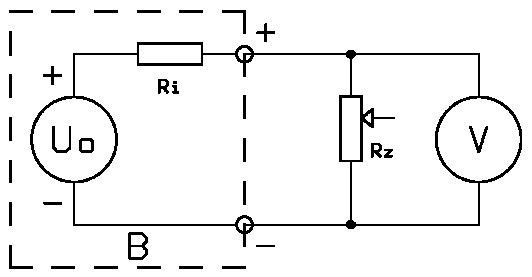
\includegraphics[scale=0.7]{schema.jpg}

\section{Postup měření}
\begin{itemize}
\item Obvod sestavíme přesně podle schématu viz schéma zapojení
\item Po zkontrolování obvodu zapneme měřicí přístroje, na dekádě nastavujeme velikost ohmické zátěže podle tabulky a zapisujeme si napětí $U$ na zátěži $R_z$
\item Poté dopočítáme podle Ohmova zákona proud $I$ protékající zátěží
\item Dopočítáme také výkon baterie do zátěže $R_z$
\item Grafickou extrapolací zjistíme napětí naprázdno $U_0$ a proud nakrátko $I_k$, dopočteme vnitřní odpor $R_i$
\item Vyneseme naměřené a dopočtené hodnoty do grafu zatšžovací charakteristiky a výkonové charakteristiky
\end{itemize}

\section{Naměřené a vypočítané hodnoty}
Hodnoty počítáme dosazením do níže uvedených vzorců.
\captionof{table}{Naměřené a vypočtené hodnoty}
\begin{tabular}{|c|c|c|c|c|c|c|c|c|c|c|c|c|}
\hline 
$R_z[\Omega]$ & 10000 & 5000 & 2500 & 1250 & 625 & 312,5 & 156,25 & 78 & 39 & 19,5 & 9,7 & 5 \\ 
\hline 
$U[V]$ & 1,46 & 1,45 & 1,42 & 1,36 & 1,26 & 1,10 & 0,88 & 0,63 & 0,41 & 0,23 & 0,13 & 0,08 \\ 
\hline 
$I[mA]$ & 0,15 & 0,29 & 0,57 & 1,09 & 2,02 & 3,52 & 5,63 & 8,08 & 10,51 & 11,8 & 13,4 & 16,0 \\ 
\hline 
$P[mW]$ & 0,22 & 0,42 & 0,81 & 1,48 & 2,55 & 3,87 & 4,95 & 5,09 & 4,31 & 2,71 & 1,74 & 1,28 \\ 
\hline
\end{tabular}
\\[0.5cm]

Pro výpočty použijeme následující vzorce:

Proud dodávaný baterií:
\begin{equation}
I = \frac{U}{R_z} \qquad [A; V, \Omega]
\end{equation}

Vnitřní odpor:
\begin{equation}
R_i = \frac{\Delta U}{\Delta I} \qquad [\Omega; V, A]
\end{equation}

Výkon baterie do zátěže $R_z$:
\begin{equation}
P = \frac{U^{2}}{R_z} = U \cdot I \qquad [W; V, \Omega]
\end{equation}

Grafickou extrapolací zjistíme, že napětí naprázdno je $U_0 = 1,64V$ a proud nakrátko je přibližně $I_k = 16mA$. Pro výpočet vnitřního odporu $R_i$ si zvolímě body v okolí bodu s největším výkonem baterie do zátěže. Poměr $R_z/R_i$ by měl být blízký hodnotě $1$. V takovém případě dodává baterie do zátěže $R_z$ největší výkon.
\begin{equation}
R_i = \frac{\Delta U}{\Delta I} = \frac{0,88 - 0,08}{16,00\cdot 10^{-3} - 5,63\cdot 10^{-3}} = 77,146\Omega
\end{equation}

\section{Grafy}
\begin{figure}[H]
\centering
	\begin{tikzpicture}
		\begin{axis}[
			width=1\textwidth,
	      	height=0.5\textwidth,
			xlabel={$I[mA]$},
			ylabel={$U[V]$}]
		\addplot[color=red,mark=x] coordinates {
			(0.15,1.46)
			(0.29,1.45)
			(0.57,1.42)
			(1.09,1.36)
			(2.02,1.26)
			(3.52,1.10)
			(5.63,0.88)
			(8.08,0.63)
			(10.51,0.41)
			(11.8,0.23)
			(13.4,0.13)
			(16.0,0.08)
		};
		\addlegendentry{$U=f(I)$}
		\addplot[color=blue,dashed] coordinates {
			(0.15,1.46)
			(16.0,1.46)
		};
		\addlegendentry{ideální}
		\end{axis}
	\end{tikzpicture}
	\caption{Zatěžovací charakteristika}
\end{figure}

\begin{figure}[H]
\centering
	\begin{tikzpicture}
		\begin{axis}[
			width=1\textwidth,
	      	height=0.6\textwidth,
			xlabel={$\frac{R_z}{R_i}[\Omega]$},
			ylabel={$P[mW]$}]
		\addplot[color=red,mark=x] coordinates {
			(99.88,0.22)
			(49.94,0.42)
			(24.97,0.81)
			(12.49,1.48)
			(6.243,2.55)
			(3.121,3.87)
			(1.561,4.95)
			(0.779,5.09)
			(0.390,4.31)
			(0.195,2.71)
			(0.097,1.74)
			(0.050,1.28)
		};
		\addlegendentry{$P=f(\frac{R_z}{R_i})$}
		\end{axis}
	\end{tikzpicture}
	\caption{Výkonová charakteristika}
\end{figure}

\section{Závěr}
Baterie dává do obvodu maximální výkon při odporu zátěže $78\Omega$ kdy výkon dosahuje více než $5mW$. To se dalo předpokládat, protože v ten okamžik dodávala baterie do obvodu největší násobek proudu a napětí. Zároveň to odpovídá o předpokladu, že pokud dodává baterie do zátěže největší výkon, měl by být poměr odporu zátěže a vnitřního odporu limitně blizký k jedné.

\section{Přístroje}
\begin{itemize}
\item Odporová dekáda č. 00167, evid. 178432
\item True RMS Digital Multimetr DM-4418 č. E0082989, evid. 109711
\item Přípravek s $1-5V$ baterií  OEM94
\end{itemize}

\end{document}
